%%%%%%%%%%%%%%%%%%%%%%%%%%%%%%%%%%%%%%%%%
% University/School Laboratory Report
% LaTeX Template
% Version 3.0 (4/2/13)
%
% This template has been downloaded from:
% http://www.LaTeXTemplates.com
%
% Original author:
% Linux and Unix Users Group at Virginia Tech Wiki 
% (https://vtluug.org/wiki/Example_LaTeX_chem_lab_report)
%
% License:
% CC BY-NC-SA 3.0 (http://creativecommons.org/licenses/by-nc-sa/3.0/)
%
%%%%%%%%%%%%%%%%%%%%%%%%%%%%%%%%%%%%%%%%%

%----------------------------------------------------------------------------------------
%	PACKAGES AND DOCUMENT CONFIGURATIONS
%----------------------------------------------------------------------------------------

\documentclass[10pt, a4paper]{article}
\usepackage[utf8x]{inputenc}
\usepackage[T1]{fontenc}
\usepackage{graphicx}
\usepackage{booktabs}
\usepackage{array}
\usepackage{longtable}
%\usepackage{anysize}
\usepackage{caption}
\usepackage{color, colortbl}
\usepackage{color}
\usepackage{amssymb}
\usepackage{amsfonts}
\usepackage{amsmath}
\usepackage{bera}% optional: just to have a nice mono-spaced font
\usepackage{listings}
\usepackage{xcolor}
\usepackage{rotating}

\colorlet{punct}{red!60!black}
\definecolor{background}{HTML}{EEEEEE}
\definecolor{delim}{RGB}{20,105,176}
\colorlet{numb}{magenta!60!black}
\PassOptionsToPackage{hyphens}{url}\usepackage{hyperref}
\hypersetup{
    pdfnewwindow=true,      % links in new window
    colorlinks=true,       % false: boxed links; true: colored links
    %urlcolor=[rgb]{0.45, 0, 0}           % color of external links
}
\definecolor{dkgreen}{rgb}{0,0.6,0}
\definecolor{gray}{rgb}{0.5,0.5,0.5}
\definecolor{light-gray}{gray}{0.95}
\definecolor{mauve}{rgb}{0.58,0,0.82}
\DeclareCaptionFont{white}{\color{white}}
\DeclareCaptionFormat{listing}{\colorbox{gray}{\parbox{\textwidth}{#1#2#3}}}
\captionsetup[lstlisting]{format=listing,labelfont=white,textfont=white}
\usepackage{listings}
\lstset{ %
                basicstyle=\ttfamily,
                keywordstyle=\color{blue}\ttfamily,
                stringstyle=\color{red}\ttfamily,
                commentstyle=\color{green}\ttfamily,
                morecomment=[l][\color{magenta}]{\#}
  basicstyle=\footnotesize,           % the size of the fonts that are used for the code
  numbers=left,                   % where to put the line-numbers
  numberstyle=\tiny\color{gray},  % the style that is used for the line-numbers
  stepnumber=1,                   % the step between two line-numbers. If it's 1, each line 
                                  % will be numbered
  numbersep=5pt,                  % how far the line-numbers are from the code
  backgroundcolor=\color{white},      % choose the background color. You must add \usepackage{color}
  showspaces=false,               % show spaces adding particular underscores
  showstringspaces=false,         % underline spaces within strings
  showtabs=false,                 % show tabs within strings adding particular underscores
  %frame=single,                   % adds a frame around the code
  rulecolor=\color{black},        % if not set, the frame-color may be changed on line-breaks within not-black text (e.g. commens (green here))
  tabsize=2,                      % sets default tabsize to 2 spaces
  captionpos=t,                   % sets the caption-position to bottom
  breaklines=true,                % sets automatic line breaking
  breakatwhitespace=false,        % sets if automatic breaks should only happen at whitespace
  title=\lstname,                   % show the filename of files included with \lstinputlisting;
                                  % also try caption instead of title
  keywordstyle=\color{blue},          % keyword style
  commentstyle=\color{dkgreen},       % comment style
  stringstyle=\color{mauve},         % string literal style
  escapeinside={\%*}{*)},            % if you want to add a comment within your code
  morekeywords={*,...}               % if you want to add more keywords to the set
}
\lstdefinelanguage{json}{
    basicstyle=\normalfont\ttfamily,
    numbers=left,
    numberstyle=\scriptsize,
    stepnumber=1,
    numbersep=8pt,
    showstringspaces=false,
    breaklines=true,
    %frame=lines,
    %backgroundcolor=\color{background},
    literate=
     *{0}{{{\color{numb}0}}}{1}
      {1}{{{\color{numb}1}}}{1}
      {2}{{{\color{numb}2}}}{1}
      {3}{{{\color{numb}3}}}{1}
      {4}{{{\color{numb}4}}}{1}
      {5}{{{\color{numb}5}}}{1}
      {6}{{{\color{numb}6}}}{1}
      {7}{{{\color{numb}7}}}{1}
      {8}{{{\color{numb}8}}}{1}
      {9}{{{\color{numb}9}}}{1}
      {:}{{{\color{punct}{:}}}}{1}
      {,}{{{\color{punct}{,}}}}{1}
      {\{}{{{\color{delim}{\{}}}}{1}
      {\}}{{{\color{delim}{\}}}}}{1}
      {[}{{{\color{delim}{[}}}}{1}
      {]}{{{\color{delim}{]}}}}{1},
}

\setlength\parindent{0pt} % Removes all indentation from paragraphs

\renewcommand{\labelenumi}{\alph{enumi}.} % Make numbering in the enumerate environment by letter rather than number (e.g. section 6)

%\usepackage{times} % Uncomment to use the Times New Roman font

%----------------------------------------------------------------------------------------
%	DOCUMENT INFORMATION
%----------------------------------------------------------------------------------------

\title{
\begin{figure}[ht]
\begin{center}

\includegraphics[scale=0.6]{./common-images/unipd_logo.pdf}
\end{center}
\end{figure}
LiES \\ Linear Equations Solver \\ Sistemi con vincoli \\\vspace{10mm} \textbf{Relazione}\\\vspace{0.4cm}
\Large{Anno Accademico 2012/2013}}

\author{Sebastiano Gottardo, Marco Ziccardi\\
Corso di studi in Informatica\\
Dipartimento di Matematica\\
Università degli Studi di Padova\\
Email: dextorer@gmail.com, marco.ziccard@gmail.com }

\date{\today} % Date for the report

\begin{document}

\maketitle % Insert the title, author and date

%\begin{center}
%\begin{tabular}{l r}
%Date Performed: & January 1, 2012 \\ % Date the experiment was performed
%Partners: & Marco Ziccardi \\ % Partner names
%& Sebastiano Gottardo \\
%\end{tabular}
%\end{center}

% If you wish to include an abstract, uncomment the lines below
% \begin{abstract}
% Abstract text
% \end{abstract}

\newpage
\tableofcontents
\newpage

%----------------------------------------------------------------------------------------
%	SECTION 1
%----------------------------------------------------------------------------------------

\section{Introduzione}
\label{sec:introduzione}

LiES (\textit{Linear Equations Solver}) e' un risolutore di sistemi di equazioni lineari, realizzato per il corso di Sistemi con Vincoli (A.A. 2012/2013). LiES permette all'utente di generare problemi di soddisfacimento di vincoli (CSP, \textit{Constraint Satisfaction Problems}) e di risolverli utilizzando diverse tecniche viste a lezione.\\

Questo documento e' strutturato nel seguente modo: dopo aver illustrato le diverse funzionalita' di LiES nella Sezione~\ref{sec:funzionalita}, verranno descritte piu' dettagliatamente le tecniche di risoluzione del sistema nella Sezione~\ref{sec:strategie}. Infine la Sezione~\ref{sec:scelte_implementative} affrontera' alcuni dettagli implementativi che risultano piu' interessanti dal punto di vista della progettazione e della realizzazione.

%----------------------------------------------------------------------------------------
%	SECTION 2
%----------------------------------------------------------------------------------------

\section{Funzionalita'}
\label{sec:funzionalita}

LiES, come risolutore di sistemi di equazioni lineari, mette a disposizione un \textbf{generatore casuale} di problemi sulla base di alcuni parametri configurabili dall'utente (per chiarezza d'esposizione, d'ora in poi ci si riferira' a sistemi di equazioni lineari con CSP). La classe dei problemi casuali generati da LiES e' della forma:
\begin{center}
	\textit{B(k,n,d,$p_1$,$p_2$)}
\end{center}

dove:
\begin{itemize}
	\item k - indica l'arieta' (numero di variabili) che caratterizza ciascun vincolo
	\item n - indica il numero di variabili
	\item d - indica la grandezza di ciascun dominio
	\item $p_1$ - indica la densita' del grafo di vincoli (ovvero, quanti vincoli rispetto al massimo)
	\item $p_2$ - indica la strettezza dei vincoli (ovvero,	quante tuple sono proibite dai vincoli) 
\end{itemize}

A partire da questi parametri, il generatore casuale di LiES genera un'istanza di problema. Tale istanza viene elaborata e visualizzata sull'apposito pannello, mentre la versione originale e' memorizzata in formato JSON (si veda listato \ref{lst:json} per un esempio).

\begin{lstlisting}[language=json, caption=Rappresentazione in formato json di un sistema di equazioni lineari, label=lst:json]
{
	"vnum": 		m,
	"cnum":			n,
	"coeffs":		[a11, a12, ..., amn],
	"cterms":		[b1, ..., bm],
	"domains":	[[l1, h1], ..., [ln, hn]]
}
\end{lstlisting}


E' altresi' possibile \textbf{esportare} un CSP su un file e \textbf{importare} un CSP precedentemente salvato; tuttavia, essendo questi CSP istanze casuali, riportare i parametri originali di creazione sarebbe superfluo e non interessante, pertanto tali parametri non vengono visualizzati.\\

Infine, LiES permette di calcolare una soluzione (se esiste) per un dato sistema di equazioni lineari generato casualmente. La scelta sul metodo di risoluzione e' lasciata all'utente, che puo' scegliere tra le seguenti tecniche:
\begin{itemize}
	\item Backtrack
	\item Bactrack, con variabile piu' vincolata
	\item Backtrack, con consistenza sugli archi
	\item Branch and bound
	\item Branch and bound, con consistenza sugli archi
\end{itemize}

La soluzione del sistema di equazioni lineari, se esistente, viene visualizzata nell'apposito pannello.

%----------------------------------------------------------------------------------------
%	SECTION 3
%----------------------------------------------------------------------------------------

\section{Strategie di risoluzione}
\label{sec:strategie}

LiES mette a disposizione cinque diverse tecniche per risolvere i sistemi di equazioni lineari generati casualmente. Gli approcci che caratterizzano ciascuna strategia sono descritte nelle successive sezioni.

\subsection{Backtrack}
\label{sec:backtrack}

La prima strategia di risoluzione disponibile è la ricerca \textit{forward checking} con \textit{backtrack}. La strategia in questione costruisce per mezzo di una funzione ricorsiva l'albero di \textit{labeling} associato al problema da risolvere. L'albero di \textit{labeling} costruito è del tipo ridotto. Un albero di \textit{labeling} ridotto necessita di un ordinamento $x_1, ..., x_n$ delle variabili del problema e viene costruito rispettando le seguenti regole:

\begin{itemize}
	\item I discendenti diretti della radice sono della forma $(x_1, d)$, ovvero partendo dal CSP originario associano un valore alla prima variabile nell'~ordinamento selezionato
	\item I discendenti diretti di un nodo $(x_j, d)$ per $i \in \left [ 1, n-1 \right ]$ sono della forma $(x_{j+1}, d)$
	\item I suoi rami determinano tutte le istanziazioni consistenti secondo l'~ordinamento $x_1, ..., x_n$ 
\end{itemize}

in questo caso nessuna tecnica di propagazione di vincoli viene utilizzata. La funzione ricorsiva responsabile per la costruzione dell'albero e ricerca di una soluzione è riportata nel listato \ref{lst:backtrack}.

\begin{lstlisting}[language=C++, caption=Funzione \texttt{solve\_rec} per la risoluzione \textit{backtrack}, label=lst:backtrack]
bool backtrack_solver_t::solve_rec(int first, int* solutions) {
     
  domain_t& domain = csp.domains[first];
  domain_t backup_domain = domain.deep_copy();
  bool solution_found = false;

  while (!domain.is_empty() && !solution_found) {
	  stats.tick();

    assignment_t assignment = domain.select_assignment();
    domain.perform_assignment(assignment);
    solutions[first] = assignment.value;
    assigned_variables[first] = 1;

    if (is_consistent(solutions)) {
      if (first+1 == csp.vnum) {
        return true;
      } else {
        solution_found = 
          solve_rec(first+1, solutions);
        if(!solution_found) {
          assigned_variables[first] = 0;
        }
      }
    }
	
	  domain.revert_assignment(assignment);
  }

  if (!solution_found) {
    domain.restore(backup_domain);
    assigned_variables[first] = 0;
  }
  return solution_found;
}
\end{lstlisting}

\setlength{\aboverulesep}{0pt}
\setlength{\belowrulesep}{0pt}
\setlength{\extrarowheight}{.75ex}
\newcolumntype{g}{>{\columncolor{light-gray}}l}
\begin{longtable}{g p{9cm}}
\toprule
\textbf{Lines 3-5} & Il dominio della variabile corrente viene salvato, sarà modificato scendendo nell'albero ma al ritorno della ricorsione esso deve poter essere ripristinato (\textit{backtrack})\\
\midrule
\textbf{Line 7} & Il ciclo assegna alla variabile corrente un valore proveniente dal dominio, l'iterazione termina quando il dominio è vuoto oppure quando in un qualche sotto-albero è stata trovata una soluzione\\
\midrule
\textbf{Lines 8} & Viene aggiornato il contatore dei nodi esaminati\\
\midrule
\textbf{Lines 10-13} & Viene selezionato un assegnamento per la variabile corrente. In questo caso si seleziona sempre il minimo valore nel dominio. In valore in questione viene rimosso dal dominio della variabile e viene temporaneamente aggiunto dell'array contenente la soluzione del problema\\
\midrule
\textbf{Line 15} & Si controlla che la soluzione finora ottenuta, seppur parziale, sia consistente\\
\midrule
\textbf{Lines 16-24} & Se l'assegnamento è consistente e la variabile assegnata è l'ultima allora è stata trovata una soluzione e la funzione ritorna \texttt{true}. Altrimenti viene invocata ricorsivamente la funzione sulla successiva variabile\\
\midrule
\textbf{Line 27} & L'assegnamento correntemente esaminato viene annullato\\
\midrule
\textbf{Lines 30-33} & Se nessuna soluzione è stata trovata nell'intero sotto-albero il dominio della variabile corrente viene ripristinato\\
\bottomrule
\end{longtable}

\subsection{Backtrack, con variabile piu' vincolata}
\label{sec:backtrack_mc}

Questa tecnica di risoluzione implementa il \textit{forward checking} con \textit{backtrack}, l'unica differenza risiede nella modalità di selezione della prossima variabile di assegnare. Nel \textit{backtrack} classico la selezione delle variabili da assegnare ad ogni livello dell'albero segue l'ordinamento $x_1, ..., x_n$. La nuova soluzione proposta implementa l'euristica per la selezione della variabile da assegnare nota come \textit{most constrained variable}. Tale euristica consiste nel selezionare la variabile non assegnata che compare nel maggior numero di vincoli. Nell'implementazione realizzata l'ordinamento di selezione delle variabili è ospitato nell'array \texttt{mc\_ordered\_variables} e calcolato in una fase di \textit{pre-processing} con la funzione mostrata nel listato \ref{lst:preprocess_mc}.

\begin{lstlisting}[language=C++, caption=Funzione \texttt{preprocess} per la risoluzione \textit{backtrack}, label=lst:preprocess_mc]
void mc_backtrack_solver_t::preprocess() {
  vector<int> variables_constraints(csp.vnum);
  unsigned int i;
  for (i = 0; i < csp.cnum; i++) {
    int* c = csp.coefs + (csp.cnum*i);
    unsigned int j;
    for (j = 0; j < csp.vnum; j++) {
      if (c[j] != 0) {
        variables_constraints[j]++;
      }
    }
  }
  for(i = 0; i < csp.vnum; i++) {
    vector<int>::iterator it = max_element(variables_constraints.begin(), variables_constraints.end());
    mc_ordered_variables[i] = distance(variables_constraints.begin(), it);
    *it = -1;   
  }
}
\end{lstlisting}

\subsection{Backtrack, con consistenza sugli archi}
\label{sec:backtrack_ac}

Questa tecnica di risoluzione realizza la ricerca \textit{backtrack} implementando la propagazione di vincoli. Prima di ricercare un assegnamento per la variabile corrente i vincoli sono propagati in modo tale da ridurre la dimensione dei domini di tutte le variabili e quindi ridurre i nodi esplorati dalla ricerca \textit{backtrack}. La propagazione di vincoli modifica il CSP originario in CSP equivalenti fino a raggiungere un criterio di consistenza; in questo caso la consistenza ricercata è quella sugli archi (\textit{arc consistency}).\\
La risoluzione usa una funzione simile a quella in listato \ref{lst:backtrack} che inoltre si occupa di ottenere la consistenza sugli archi per mezzo della funzione in listato \ref{lst:propagate}. \texttt{propagate} implementa l'argoritmo di consistenza sugli archi \texttt{AC-3}, che ha complessità $O(ek^3)$ dove $e$ è il numero di vincoli nel problema e $l$ è la dimensione dei domini.\\
Nel nostro caso specifico i domini non sono altro che intervalli di interi e sono rappresentati nel programma tramite una collezione di intervalli ($\left [ l, h \right ]$). Si noti che ciascun dominio è una collezione di intervalli di interi in quanto possibili estensioni future potrebbero richiedere la rimozione dal dominio di elementi nel mezzo dell'intervallo con conseguente necessità di suddividere quest'ultimo.\\
In una fase di \textit{pre-processing} tutti i vincoli binari del problema sono raccolti in una collezione \texttt{binary\_constraints} poi utilizzata dalla funzione \texttt{propagate}.

\begin{lstlisting}[language=C++, caption=Funzione \texttt{propagate} che rende un CSP consistente sugli archi, label=lst:propagate]
void ac_backtrack_solver_t::propagate() {
  vector<binary_constraint_t> constraints = binary_constraints;
  
  while (!constraints.empty()) {
    vector<binary_constraint_t>::iterator constraint = constraints.begin();

    int cterm = csp.cterms[constraint->id];
    int* c = csp.coefs + (csp.cnum * (constraint->id));
    domain_t& domain1 = csp.domains[constraint->var1];
    domain_t& domain2 = csp.domains[constraint->var2];
    bool domain_changed = false;
    unsigned int interval1_id;
    for (interval1_id = 0; interval1_id < domain1.intervals.size(); interval1_id++) {
      interval_t& interval1 = domain1.intervals[interval1_id];
      int value1;
      for (value1 = interval1.l; value1 <= interval1.h; value1++) {
        bool consistent = false;
        vector<interval_t>::iterator interval2;
        unsigned int interval2_id;
        for (interval2_id = 0; interval2_id < domain2.intervals.size() && !consistent; interval2_id++) {
          interval_t& interval2 = domain2.intervals[interval2_id];
          int value2;
          for (value2 = interval2.l; value2 <= interval2.h; value2++) {
            if ((c[constraint->var1]*value1) == (cterm - c[constraint->var2]*value2)) {
              consistent = true;
            }
          }
        }
        if (!consistent) {
          domain_changed = true;

          // Remove value1 from the domain
          domain1.split(interval1_id, value1);
        }            
      }   
    }
    if (domain_changed) {
      vector<binary_constraint_t>::iterator new_constraint;
      for (new_constraint = binary_constraints.begin(); new_constraint != binary_constraints.end(); new_constraint++) {
        if (constraint->var1 == new_constraint->var2) {
          bool found = false;
          unsigned int i;
          for (i = 0; i < constraints.size() && !found; i++) {
            if (constraints[i].id == new_constraint->id && 
              constraints[i].var1 == new_constraint->var1 && 
              constraints[i].var2 == new_constraint->var2) {
              found = true;
            }
          }
          if (!found) { 
            constraints.push_back(*new_constraint); 
          }
        }
      }
    }
    constraints.erase(constraint);        
  }
}
\end{lstlisting}

\setlength{\aboverulesep}{0pt}
\setlength{\belowrulesep}{0pt}
\setlength{\extrarowheight}{.75ex}
\newcolumntype{g}{>{\columncolor{light-gray}}l}
\begin{longtable}{g p{9cm}}
\toprule
\textbf{Line 2} & Viene creata una collezione che contiene tutti i vincoli binari la cui consistenza sugli archi deve ancora essere controllata\\
\midrule
\textbf{Line 4} & Si itera finchè la collezione di vincoli binari non è vuota\\
\midrule
\textbf{Line 4} & Si itera finchè la collezione di vincoli binari non è vuota\\
\midrule
\textbf{Lines 5-12} & Per ciascun vincolo binario selezionato si identificano i domini delle variabili coinvolte, siano esse $x_1$ e $x_2$\\
\midrule
\textbf{Lines 13-19} & Si itera su ciascun possibile valore della variabile $x_1$\\
\midrule
\textbf{Lines 20-23} & Si itera su ciascun possibile valore della variabile $x_2$\\
\midrule
\textbf{Lines 24-26} & Si controlla che il vincolo selezionato sia consistente sui valori selezionati\\
\midrule
\textbf{Lines 29-34} & Nel caso in cui per nessun valore della variabile $x_2$ il valore della variabile $x_1$ verifica il vincolo selezionato esso va rimosso dal dominio di $x_1$ e tale dominio viene marcato come modificato\\
\midrule
\textbf{Lines 37-55} & Qualora il dominio di $x_1$ sia cambiato vanno inseriti nella collezione di vincoli da esaminare tutti quelli che coinvolgono una qualsiasi variabile $x_j$ con $j\neq1$ e $x_1$\\
\midrule
\textbf{Line 56} & Il vincolo appena considerato viene eliminato dalla collezione\\
\bottomrule
\end{longtable}

\subsection{Branch and bound}
\label{sec:branch_and_bound}

Passiamo ora alle tecniche di ricerca di una soluzione ottima. La prima tecnica implementata è quella che realizza un semplice \textit{branch and bound}. La ricerca \textit{branch and bound} costruisce un albero di ricerca esattamente come la ricerca \textit{backtrack} ma non si ferma alla prima soluzione consistente, ricerca invece la soluzione ottima secondo una data funzione obiettivo $f$. La ricerca mantiene inoltre che un valore $bound$ che rappresenta il valore della funzione obiettivo per la migliore soluzione trovata finora. In combinazione al valore $bound$ si usa una funzione euristica che valuti la qualità di soluzioni incomplete, la funzione euristica $h$ è tale da permetterci di escludere dalla ricerca l'intero sotto-albero qualora il valore di $h$ per il nodo visitato sia già peggiore di $bound$.\\
Nel nostro caso la funzione obiettivo usata corrisponde alla somma delle variabili di indice pari:
\begin{equation*}
f(X) = \sum_{i \in [0,n-1]:~i~is~even} x_i
\end{equation*}
E vogliamo ottenere la soluzione che minimizza il valore $f(X)$, a questo scopo usiamo come funzione euristica:
\begin{equation*}
h(X) = \sum_{i \in [0,n-1]:~i~is~even} min(x_i)
\end{equation*}
Dove $min(x_i)$ è il valore assegnato a $x_i$ se la variabile è stata istanziata, altrimenti è il minimo valore assegnabile a $x_i$ proveniente dal suo dominio. Date le suddette funzioni, qualora si trovi una soluzione tale che $f(X) < bound$ allora $bound$ viene aggiornata e qualora si incontri un nodo tale che $h(X) \geq bound$ allora l'intero sottoalbero viene escluso dalla ricerca.\\
La funzione che si occupa della ricerca \textit{branch and bound} è riportata in listato \ref{lst:bb_solve_rec}

\begin{lstlisting}[language=C++, caption=Funzione \texttt{solve\_rec} per la risoluzione \textit{branch and bound}, label=lst:bb_solve_rec]
bool bb_solver_t::solve_rec(int first, int* solutions){
  if (evaluate_node(solutions, first) > min_value) {
    return true;
  }
 
  domain_t& domain = csp.domains[first];
  domain_t backup_domain = domain.deep_copy();

  while (!domain.is_empty()) {
    assignment_t assignment = domain.select_assignment();
    domain.perform_assignment(assignment);

    solutions[first] = assignment.value;
    assigned_variables[first] = 1;

    stats.tick();

    if (is_consistent(solutions)) {
      if (first+1 == csp.vnum) {
        long evaluation = evaluate_node(solutions, first);
        if (evaluation < min_value) {
          min_value = evaluation;
          memcpy(min_solutions,solutions,csp.vnum*sizeof(int));
        }
      } else { 
        solve_rec(first+1, solutions);
      }
    }
    assigned_variables[first] = 0;
    domain.revert_assignment(assignment);
  }
  domain.restore(backup_domain);
  assigned_variables[first] = 0;
  return true;
}
\end{lstlisting}

\setlength{\aboverulesep}{0pt}
\setlength{\belowrulesep}{0pt}
\setlength{\extrarowheight}{.75ex}
\newcolumntype{g}{>{\columncolor{light-gray}}l}
\begin{longtable}{g p{9cm}}
\toprule
\textbf{Lines 2-4} & Se la valutazione euristica del nodo corrente è maggiore del miglior valore della funzione obiettivo finora ottenuto (\texttt{min\_value}) la funzione ritorna, scartando l'intero sottoalbero\\
\midrule
\textbf{Lines 6-7} & Il dominio della variabile corrente viene salvato, sarà modificato scendendo nell'albero ma al ritorno della ricorsione esso deve poter essere ripristinato\\
\midrule
\textbf{Line 9} & Il ciclo assegna alla variabile corrente un valore proveniente dal dominio, l'iterazione termina quando il dominio è vuoto\\
\midrule
\textbf{Lines 10-14} & Viene selezionato un assegnamento per la variabile corrente. In questo caso si seleziona sempre il minimo valore nel dominio. In valore in questione viene rimosso dal dominio della variabile e viene temporaneamente aggiunto dell'array contenente la soluzione del problema\\
\midrule
\textbf{Line 16} & Viene aggiornato il contatore dei nodi esaminati\\
\midrule
\textbf{Line 18} & Si controlla che la soluzione finora ottenuta, seppur parziale, sia consistente\\
\midrule
\textbf{Lines 19-27} & Se l'assegnamento è consistente e la variabile assegnata è l'ultima allora è stata trovata una soluzione. Si calcola la funzione obiettivo sulla soluzione appena trovata e qualora sia minore di \texttt{min\_value} si aggiorna questo valore e la soluzione ottima \texttt{min\_solutions}. Se la variabile assegnata non è l'ultima si invoca ricorsivamente la funzione sulla variabile successiva\\
\midrule
\textbf{Lines 29-30} & L'assegnamento correntemente esaminato viene annullato\\
\midrule
\textbf{Line 32} & Se nessuna soluzione è stata trovata nell'intero sotto-albero il dominio della variabile corrente viene ripristinato\\
\bottomrule
\end{longtable}

\subsection{Branch and bound, con consistenza sugli archi}
\label{sec:branch_and_bound_ac}

Questa tecnica di risoluzione realizza la ricerca \textit{branch and bound} implementando la propagazione di vincoli. Prima di ricercare un assegnamento per la variabile corrente i vincoli sono propagati in modo tale da ridurre la dimensione dei domini di tutte le variabili e quindi ridurre i nodi esplorati dalla ricerca \textit{branch and bound}. La propagazione di vincoli modifica il CSP originario in CSP equivalenti fino a raggiungere un criterio di consistenza; in questo caso la consistenza ricercata è quella sugli archi (\textit{arc consistency}).\\
La ricerca viene realizzata per mezzo di una funzione simile a quella riportata in listato \ref{lst:bb_solve_rec} mentre la consistenza sugli archi viene garantita dalla funzione in listato \ref{lst:propagate}.

%----------------------------------------------------------------------------------------
%	SECTION 4
%----------------------------------------------------------------------------------------

\section{Test}

Gli algorimti di risoluzione sono stati testati da riga di comando e diversi dati sono stati raccolti al fine di analizzarne il comportamento. I primi dati raccolti sono relativi ad una esecuzione degli algoritmi \textit{backtrack}, \textit{backtrack} con euristica \textit{most constrained variable} e \textit{backtrack} con \textit{arc consistency} su un semplice problema in 3 variabili. La seconda batteria di test eseguita studia il comportamento dei tre precedenti algoritmi su problemi generati casualmente all'aumentare del numero di variabili. Infine sono stati raccolti tempi di esecuzione e numero di nodi visitati per gli algoritmi \textit{branch and bound} e \textit{branch and bound} con \textit{arc consistency}.

\subsection{Test 1}
Gli algoritmi \textit{backtrack} (\texttt{Backtrack}), \textit{backtrack} con euristica \textit{most constrained variable} (\texttt{MC\_Backtrack}) e \textit{backtrack} con \textit{arc consistency} (\texttt{AC\_Backtrack}) sono stati eseguiti sul problema riportato in listato \ref{lst:csp1}.

\begin{lstlisting}[language=json, caption=csp1: problema sul quale è stata eseguita la prima batteria di test, label=lst:csp1]
{
	"vnum": 		3,
	"cnum":			3,
	"coeffs":		[1, 0, 1, 1, 0, 1, 0, 1, 0],
	"cterms":		[10, 10, 5],
	"domains":	[[-10, 10], [0, 10], [0, 10]]
}
\end{lstlisting}

I dati raccolti sono relativi a tempi di esecuzione e nodi visitati dai vari algoritmi i sono riportati in tabella \ref{tab:test1}.

\begin{longtable}{c c c}
\toprule
\textbf{Algorithm} & \textbf{Time (ms)} & \textbf{Nodes}\\
\midrule
\texttt{Backtrack} & 0,515 & 248 \\
\midrule
\texttt{MC\_Backtrack} & 0,295 & 138 \\
\midrule
\texttt{AC\_Backtrack} & 0,075 & 8 \\
\bottomrule
\caption{Tempi di esecuzione e numero di nodi visitati nella ricerca di una soluzione al problema csp1}
\label{tab:test1}
\end{longtable}

\begin{figure}[!h]
\begin{center}
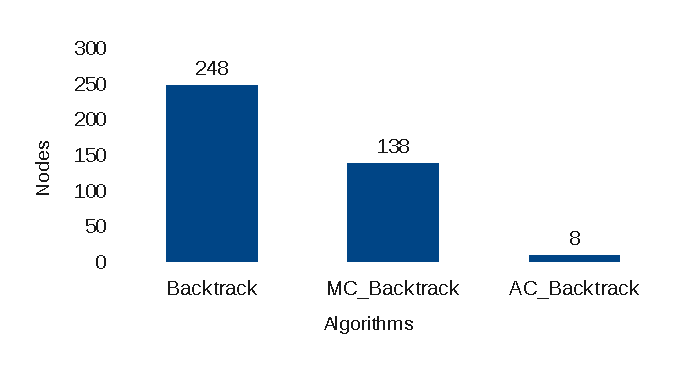
\includegraphics[scale=0.7]{./report-images/test1_nodes.pdf}
\caption{Grafico dei nodi visitati nella risoluzione del problema csp1}
\label{fig:test1_nodes}
\end{center}
\end{figure}

Nelle figure \ref{fig:test1_nodes} e \ref{fig:test1_time} si può notare come sia il numero di nodi che il tempo di esecuzione diminuiscano usando l'algoritmo \texttt{MC\_backtrack} rispetto all'algoritmo \texttt{Backtrack}. \texttt{MC\_backtrack} infatti, assegnando per prime le variabili che compaiono in più vincoli permette di restringere maggiormente il dominio delle successive variabili da assegnare, riducendo la dimensione dell'albero da visitare. Come atteso l'algoritmo migliore si rivela \texttt{AC\_backtrack} che riduce al minimo la quantità di nodi da visitare rimpicciolendo i domini tramite la consistenza sugli archi.

\begin{figure}[!h]
\begin{center}
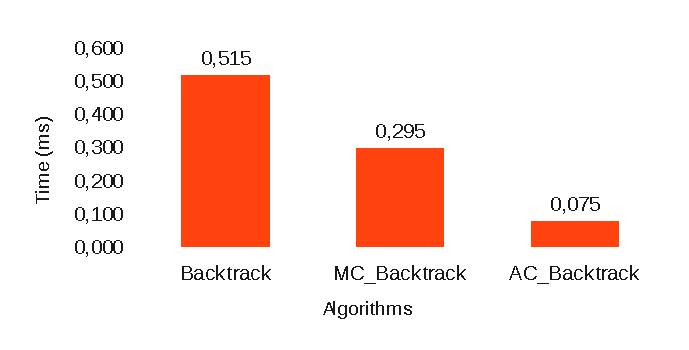
\includegraphics[scale=0.7]{./report-images/test1_time.pdf}
\caption{Grafico dei tempi di esecuzione nella risoluzione del problema csp1}
\label{fig:test1_time}
\end{center}
\end{figure}

\subsection{Test 2}

\begin{sidewaystable}
\centering
\begin{tabular}{c | c | c | c c | c c | c c}
\textbf{Problem} & \textbf{Variables} & \textbf{Status} & \multicolumn{2}{c}{\textbf{Backtrack}} & \multicolumn{2}{c}{\textbf{MC\_Backtrack}} & \multicolumn{2}{c}{\textbf{AC\_Backtrack}} \\
 & & & \textbf{Nodes} & \textbf{Times (ms)} & \textbf{Nodes} & \textbf{Times (ms)} & \textbf{Nodes} & \textbf{Times (ms)}\\
\toprule
cspa.json & SOLVED & 4 & 1267 & 653,435 & 67 & 11,714 & 4 & 3,394 \\
\midrule
cspb.json & FAILED & 5 & 8840 & 8217,945 & 8840 & 9376,913 & 8422 & 7755,468 \\
\midrule
cspc.json & FAILED & 6 & 168420 & 118,939 & 8420 & 6,66 & 0 & 0,025 \\
\midrule
cspe.json & FAILED & 7 & 3368420	& 3443,583 & 8420 & 7,329 & 0 & 1,952 \\
\midrule
cspd.json & FAILED & 8 & 168420 & 263,697 & 420 & 1,877 & 0 & 0,096 \\
\midrule
cspf.json & FAILED & 9 & 3368420	& 2732,075 & 420 & 1,279 & 0 & 0,031 \\
\midrule
cspg.json & FAILED & 10 & 168420	& 161,748 & 8420 & 7,275 & 0 & 0,038 \\
\midrule
csph.json & FAILED & 11 & 3368420 & 6513,557 & 168420 & 155,434 & 0 & 0,035 \\
\midrule
cspi.json & FAILED & 12 & 176820	& 243,419 & 168420 & 228,973 & 0 & 0,036 \\
\bottomrule
\end{tabular}
\caption{Numero di nodi visitati e tempi di esecuzione della risoluzione di problemi generati casualmente all'aumentare del numero di variabili}
\label{tab:test2}
\end{sidewaystable}

Gli algoritmi \textit{backtrack} (\texttt{Backtrack}), \textit{backtrack} con euristica \textit{most constrained variable} (\texttt{MC\_Backtrack}) e \textit{backtrack} con \textit{arc consistency} (\texttt{AC\_Backtrack}) sono stati eseguiti su un insieme di 9 problemi generati casualmente a partire dai parametri \texttt{(2, n, 20, 0.2, 0.5)} con n crescente da $4$ a $12$. I problemi (da \texttt{cspa} a \texttt{cspi}) sono disponibili al seguente indirizzo \url{https://github.com/mziccard/LiES/csolver/test}.\\
Numero di nodi visitati e tempi di esecuzione raccolti sono mostrati in tabella \ref{tab:test2}.



Come si nota dalla tabella \ref{tab:test2} l'algoritmo \texttt{AC\_Backtrack} spesso risolve il problema ancor prima di iniziare la ricerca di una soluzione: in questi casi la propagazione di vincoli fino alla consistenza sugli archi svuota il dominio di qualche variabile, rendendo inutile ogni tentativo di risoluzione, il problema non ha soluzione. Dai dati notiamo inoltre come la complessità di un problema non dipenda esclusivamente dal numero di variabili ma essa dipende inoltre dalla complessita intrinseca del problema (strettezza dei vincoli).\\ Dai dati vediamo inoltre come i tempi di esecuzione e il numero di nodi visitati tenda a crescere (salvo oscillazioni imputabili alla complessita intrinseca di alcuni problemi) in maniera esponenziale al crescere del numero di variabili. Come atteso \texttt{MC\_Backtrack} si comporta meglio di \texttt{Backtrack}, limitando notevolemente il numero di nodi visitati e il tempo di esecuzione. Anche in questo caso tuttavia l'andamento del numero di nodi visitati al crescere del numero di variabili sembra essere esponenziale. I problemi generati casualmente hanno tutti vincoli di arietà pari a 2 e quindi ci aspettavamo che l'algoritmo che assicurasse le prestazioni migliori fosse \texttt{AC\_\allowbreak Backtrack} (dal momento che la consistenza sugli archi riduce i domini a partire da vincoli binari). Dati alla mano, infatti, \texttt{AC\_Backtrack} si conferma essere l'algoritmo migliore.\\
In figura \ref{fig:test2_nodes} è rappresentato per ciascuno dei tre algoritmi il logaritmo in base dieci del numero di nodi visualizzati $(log(nodes))$. Rappresentiamo il logaritmo del numero di nodi e non il numero di nodi stesso per rendere la visualizzazione più efficace. Nel caso di \texttt{AC\_Backtrack}, in cui il numero di nodi visualizzati è $0$, normalizziamo anche il logaritmo a $0$.

\begin{figure}[!h]
\begin{center}
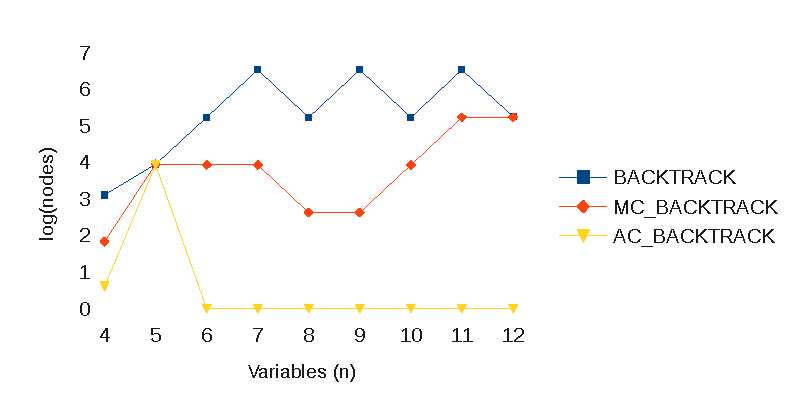
\includegraphics[scale=0.8]{./report-images/test2_nodes.pdf}
\caption{Grafico dei nodi visitati nella risoluzione di problemi generati casualmente all'aumentare del numero di variabili}
\label{fig:test2_nodes}
\end{center}
\end{figure}

Notiamo dal grafico in figura \ref{fig:test2_nodes} che il logaritmo dei nodi visitati sembra crescere linearmente per gli algoritmi \texttt{Backtrack} e \texttt{MC\_Backtrack}. Ciò significa che, come atteso, il numero di nodi visitati cresce esponenzialmente al crescere del numero di variabili per questi due algoritmi. L'algoritmo \texttt{AC\_Backtrack} si rivela notevolmente migliore, principalmente a causa del fatto che tutti i vincoli nei problemi sono binari e la consistenza sugli archi in questi casi è particolarmente efficace.\\
In figura \ref{fig:test2_time} riportiamo invece l'andamento dei tempi di esecuzione dei vari algoritmi al crescere del numero di variabili. Da entrambi i grafici \ref{fig:test2_nodes} e \ref{fig:test2_time} riportati notiamo come il problema \texttt{cspb} in $5$ variabili risulti particolarmente complesso per tutti gli algoritmi.

\begin{figure}[!h]
\begin{center}
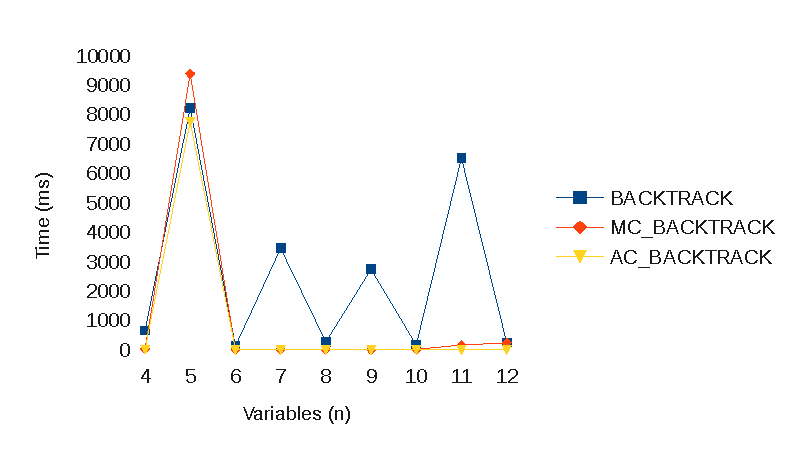
\includegraphics[scale=0.9]{./report-images/test2_time.pdf}
\caption{Grafico dei tempi di esecuzione nella risoluzione di problemi generati casualmente all'aumentare del numero di variabili}
\label{fig:test2_time}
\end{center}
\end{figure}

\subsection{Test 3}
Gli algoritmi \textit{branch and bound} (\texttt{BB}), \textit{branch and bound} con \textit{arc consistency} (\texttt{AC\_BB}) sono stati eseguiti sul problema riportato in listato \ref{lst:csp1}.\\
I dati raccolti sono relativi a tempi di esecuzione e nodi visitati dai vari algoritmi i sono riportati in tabella \ref{tab:test2}.

\begin{longtable}{c c c}
\toprule
\textbf{Algorithm} & \textbf{Time (ms)} & \textbf{Nodes}\\
\midrule
\texttt{BB} & 344,155 & 483 \\
\midrule
\texttt{AC\_BB} & 9,926 & 23 \\
\bottomrule
\caption{Tempi di esecuzione e numero di nodi visitati nella ricerca di una soluzione ottima al problema csp1}
\label{tab:test2}
\end{longtable}

Nei grafici in figura \ref{fig:test3_nodes} e \ref{fig:test3_time} sono riportati rispettivamente i nodi visitati e i tempi di esecuzione per gli algoritmi \textit{branch and bound} e \textit{branch and bound} con \textit{arc consistency}. Come atteso \texttt{BB\_AC} è notevolmente più veloce del semplice \texttt{BB}, la consistenza sugli archi nel caso in cui si debba percorrere tutto l'albero alla ricerca di una soluzione ottima porta vantaggi prestazionali ancora più sensibili.

\begin{figure}[!h]
\begin{center}
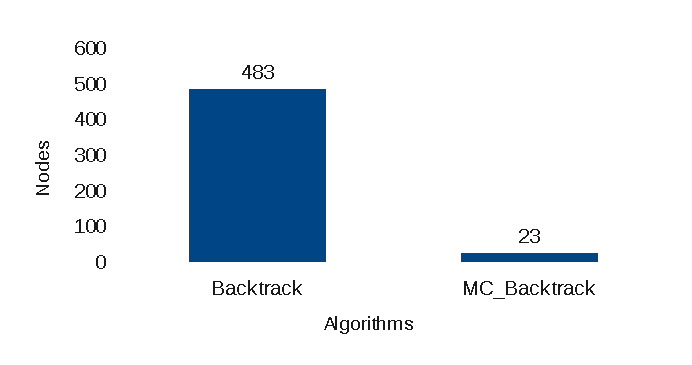
\includegraphics[scale=0.7]{./report-images/test3_nodes.pdf}
\caption{Grafico dei nodi visitati nella risoluzione ottima del problema csp1}
\label{fig:test3_nodes}
\end{center}
\end{figure}

\begin{figure}[!h]
\begin{center}
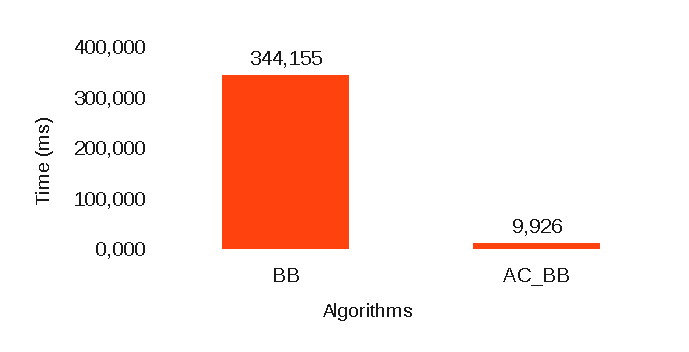
\includegraphics[scale=0.7]{./report-images/test3_time.pdf}
\caption{Grafico dei tempi di esecuzione nella risoluzione ottima del problema csp1}
\label{fig:test3_time}
\end{center}
\end{figure}

\section{Scelte implementative}
\label{sec:scelte_implementative}

LiES e' stato progettato per essere al tempo stesso performante e graficamente gradevole. Questi requisiti hanno portato ad un approccio ibrido per quanto riguarda i linguaggi di programmazione ed i framework utilizzati. Il risolutore e' stato scritto utilizzando il \textbf{linguaggio C} a causa della sua estrema efficienza in termini di calcolo puro. Inoltre, grazie ad elementi come le \verb+struct+, e' possibile avere una modellazione simil-object-oriented senza pero' introdurre maggiore complessita' di calcolo.\\

Per quanto riguarda la User Interface (UI), la scelta e' invece ricaduta sul \textbf{linguaggio Java}, che grazie alle librerie grafiche \textit{Swing} e \textit{AWT} permette di creare interfacce grafiche il cui aspetto e' indipendente dalla piattaforma d'esecuzione e pertanto mantiene la stessa esperienza d'uso.\\

Ad ogni modo, i linguaggi Java e C non sono interoperabili, richiedendo quindi una soluzione che permettesse una comunicazione bi-direzionale tra la UI e il risolutore. Sono state prese in considerazione due alternative:
\begin{itemize}
	\item JNI (\textit{Java Native Interface}) - si tratta di un framework che permette ad applicazioni Java di chiamare (ed essere chiamate da) codice nativo, in questo caso codice C
	\item Runtime execution - e' possibile invocare comandi ``nativi'' (i.e., propri del sistema operativo) direttamente dalla runtime di Java
\end{itemize}

Nonostante JNI offra un meccanismo molto valido per l'invocazione di codice nativo, la scelta e' ricaduta sulla seconda opzione, piu' semplice ed immediata.

%----------------------------------------------------------------------------------------
%	SECTION 5
%----------------------------------------------------------------------------------------

\section{Requisiti di funzionamento}
\label{sec:requisiti_funzionamento}

In base a quanto riportato in Sezione~\ref{sec:scelte_implementative}, vi sono due requisiti fondamentali affinche' LiES funzioni correttamente, riportati di seguito:
\begin{itemize}
	\item Presenza di una JVM/JRE - in altre parole, il sistema operativo deve essere in grado di eseguire applicazioni Java
	\item Presenza di un compilatore C - in maniera tale da poter compilare il risolutore
\end{itemize}

Come descritto dal manuale utente, uno script si occupera' di automatizzare il processo di compilazione del risolutore, gia' reso molto semplice dalla presenza di un \verb+makefile+.

%----------------------------------------------------------------------------------------
%	SECTION 6
%----------------------------------------------------------------------------------------

\section{Versionamento}
\label{sec:versionamento}

Tutto il codice inerente lo sviluppo di LiES e' stato versionato in un repository pubblico su GitHub, un famosissimo portale di social coding. Come si evince dal nome, il sistema di versionamento utilizzato e' \verb+git+.\\

L'URL del suddetto repository e' il seguente: \url{https://github.com/mziccard/LiES}.

%----------------------------------------------------------------------------------------


\end{document}
